\problemname{Forest for the Trees}

You are playing hide-and-go-seek in a forest with Belle.  The forest
has one tree at each of the positive integer lattice points.  That is,
there is a tree at every point $(x,y)$ where $x$ and $y$ are both
positive integers.  You may consider each tree as a point.  A logging
company has cut down all of the trees in some axis-aligned rectangle,
including those on the boundary of the rectangle.

You are standing at $(0,0)$ and Belle is standing at $(x_b,y_b)$.
You can see Belle if and only if there is no tree blocking your line of
sight to Belle. If there is a tree at $(x_b,y_b)$, Belle will make
it easier for you to find her by standing on the side of the tree
facing your location.

For example, suppose that Belle is standing at $(2,6)$.  If the
trees in the rectangle with corners at $(1,1)$ and $(5,4)$ are cut
down (blue rectangle in figure), then you can see Belle.  However,
if the rectangle was at $(3,5)$ and $(5,7)$ (red rectangle in figure),
then the tree at $(1,3)$ would be in the way.

\begin{center}
	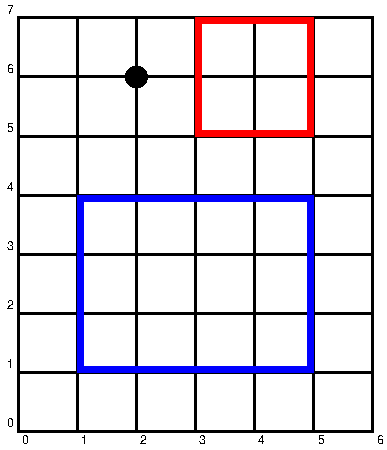
\includegraphics[width=0.45\textwidth]{trees.pdf}
\end{center}

Given the rectangle and Belle's location, can you see her?

\section*{Input}

The first line of input contains two integer $x_b$ and $y_b$~($1 \leq x_b,y_b \leq 10^{12}$), which are the coordinates that Belle is 
standing on.

The second line of input contains four integers $x_1$, $y_1$, $x_2$ and $y_2$~($1 \leq x_1 \leq x_2 \leq 10^{12}$ and $1 \leq y_1 \leq y_2 
\leq 10^{12}$), which specify two opposite corners of the rectangle at $(x_1, y_1)$ and $(x_2, y_2)$.

\section*{Output}

If you can see Belle, display \texttt{Yes}.

Otherwise, display \texttt{No} and the coordinates of the closest tree
that is blocking your view.
